% -*- TeX -*-
\documentclass{beamer}

\usepackage{amsmath}
\usepackage{array}
\usepackage{tikz}

\usetikzlibrary{decorations.pathreplacing}
\usetikzlibrary{fit,matrix}
\defbeamertemplate{description item}{align left}{\insertdescriptionitem\hfill}

\title{Crustal Deformation Modeling Tutorial}
\subtitle{Static Green's Functions}
\author{Charles Williams \\
  Brad Aagaard \\
  Matthew Knepley}
\institute{
\includegraphics[scale=0.4]{../../logos/cig_blackfg}}
\date{June 21, 2022}


% ---------------------------------------------------- CUSTOMIZATION
\renewcommand{\thispdfpagelabel}[1]{}
\newcommand{\pylith}[1]{{\color{green}#1}}
\newcommand{\python}[1]{{\color{red}#1}}
\usetheme{CIG}

\newcommand{\tensor}[1]{\overline{#1}}

% ========================================================= DOCUMENT
\begin{document}

% ------------------------------------------------------------ SLIDE
\maketitle

% ------------------------------------------------------------ SLIDE
\logo{
\includegraphics[height=4.5ex]{../../logos/cig_blackfg}}

% ========================================================== SECTION
\section{Static Green's Functions}

% ========================================================== SUBSECTION
\subsection{Concepts covered}
% ------------------------------------------------------------ SLIDE
\begin{frame}
  \frametitle{Concepts Covered in this Session}
  \summary{}

  \begin{itemize}
  \item Generation of simple mesh using Gmsh and/or Cubit
  \item Generation of randomly located synthetic GPS stations using
    \python{numpy}
  \item Simulation of a coseismic event in 2D
  \item Generation of static Green's functions
  \item Simple inversion of synthetic data using \python{numpy}
  \item Plotting of inversion results using \python{matplotlib} and
    \python{h5py}
  \end{itemize}
  
\end{frame}

% ========================================================== SECTION
\subsection{Files used for simulations}

% ------------------------------------------------------------ SLIDE
\begin{frame}
  \frametitle{Files used in simulations}
  \summary{Files are in directory \python{examples/strikeslip-2d}}

  \setbeamertemplate{description item}[align left]
  \begin{description}
  \item[README.md] README file with brief description of examples.
  \item[*.cfg] PyLith parameter files.
  \item[generate\_gmsh.py] Python script to generate mesh using Gmsh.
  \item[generate\_gpsstations.py] Python script to generate synthetic
    GPS sites.
  \item[invert\_slip.py] Python script to invert synthetic data for
    fault slip.
  \item[*.msh] Gmsh finite-element mesh files generated by Gmsh.
  \item[*.jou] Files used to construct mesh using Cubit.
  \item[*.exo] Exodus II mesh files generated by Cubit.
  \item[*.spatialdb] Files associated with the spatial databases.
  \item[viz] Directory containing ParaView Python scripts and other
    files for visualizing results.
  \item[output] Directory containing simulation output.
  \end{description}

\end{frame}

% ========================================================== SUBSECTION
\subsection{Overview}

% ------------------------------------------------------------ SLIDE
\begin{frame}
  \frametitle{Green's Functions}
  \summary{}

  \begin{itemize}
  \item Compute deformation due to unit (i.e., 1 m) slip at fault
    vertices for use in an inversion for fault slip
    \begin{itemize}
    \item Slip decreases {\bf linearly} to 0 at surrounding vertices
    \item Similar but not equivalent to uniform slip over a patch
      (Okada dislocation)
    \item PyLith interpolates the responses to user-specified points
      using \pylith{OutputSolnPoints} output manager
    \end{itemize}
  \item Provides ability to compute Green's functions with arbitrarily
    complex elastic structure and/or topography
  \end{itemize}
  
\end{frame}

% ========================================================== SECTION
\subsection{Basic layout for simulations}

% ------------------------------------------------------------ SLIDE
\begin{frame}
  \frametitle{Two-dimensional Strike-slip Simulations}
  \summary{}

  \vfill
  \begin{center}
      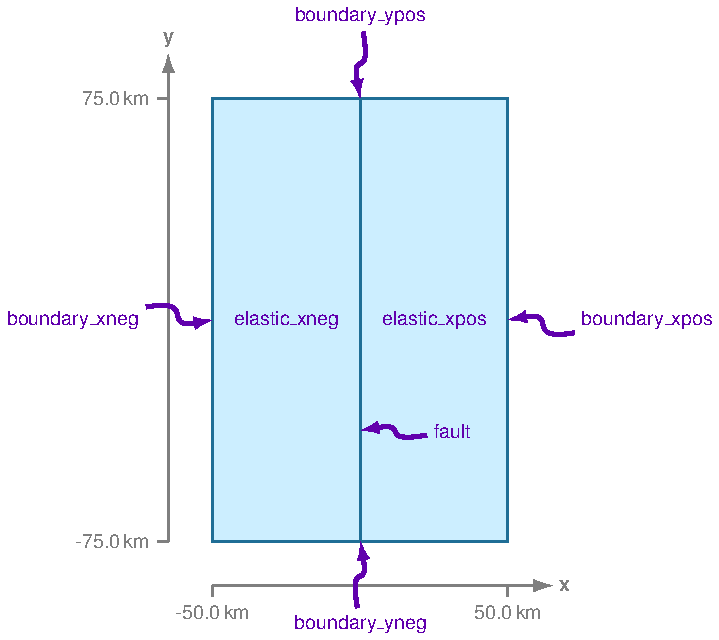
\includegraphics[height=6.1cm]{figs/geometry}
  \end{center}
  \vfill

\end{frame}

% ========================================================== SECTION
\subsection{step04-varslip}

% ------------------------------------------------------------ SLIDE
\begin{frame}
  \frametitle{Step 04}
  \summary{Variable coseismic slip applied to elastic material}

  \vfill
  \begin{center}
      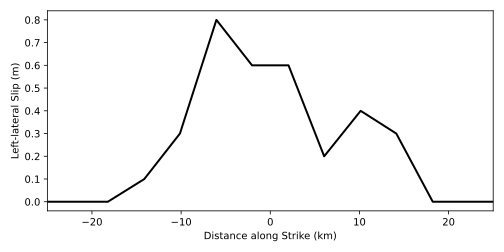
\includegraphics[height=6.1cm]{figs/step04-slip}
  \end{center}
\vfill
      
\end{frame}


% ========================================================== SECTION
\subsection{Linear inversion}

% ------------------------------------------------------------ SLIDE
\begin{frame}
  \frametitle{Simple Linear Inversion}
  \summary{Parameters}

  \begin{description}
  \item[\textit{G}] Green's function matrix
  \item[\textit{d}] Unknown fault slip
  \item[\begin{math}d_{apriori}\end{math}] A priori estimate of fault slip
  \item[\begin{math}u_{obs}\end{math}] Observed displacement
  \item[\textit{D}] Penalty matrix
  \item[\begin{math}\theta\end{math}] Penalty parameter
  \end{description}
  
  \vfill The matrix \begin{math}{G_{ij}}\end{math} gives displacement
  component \textit{i} due to a unit of slip from component \textit{j}.
\vfill

\end{frame}


% ------------------------------------------------------------ SLIDE
\begin{frame}
  \frametitle{Simple Linear Inversion}
  \summary{Equations}

  \begin{itemize}
  \item Original system of equations:
    \begin{equation}
      G d = u_{obs}
    \end{equation}

  \item Augmented system of equations:
    \begin{equation}
      G_a d = u_a \text{, where } 
      G_a = \left[ \begin{array}{c} G \\ \theta D \end{array} \right]
      \text{ and }
      u_a = \left[ \begin{array}{c} u_{obs} \\ d_{apriori} \end{array} \right]
    \end{equation}
    
  \item Generalized inverse:
    \begin{gather}
      G^{-g} = \left( G_a^T G_a \right)^{-1} G_a^T \\
      d_{est} = G^{-g} u_a
    \end{gather}
  \end{itemize}
  
\end{frame}


% ========================================================== SECTION
\subsection{Inversion results}

% ------------------------------------------------------------ SLIDE
\begin{frame}
  \frametitle{Inversion results}
  \summary{Predicted slip distribution}

  \vfill
  \begin{center}
    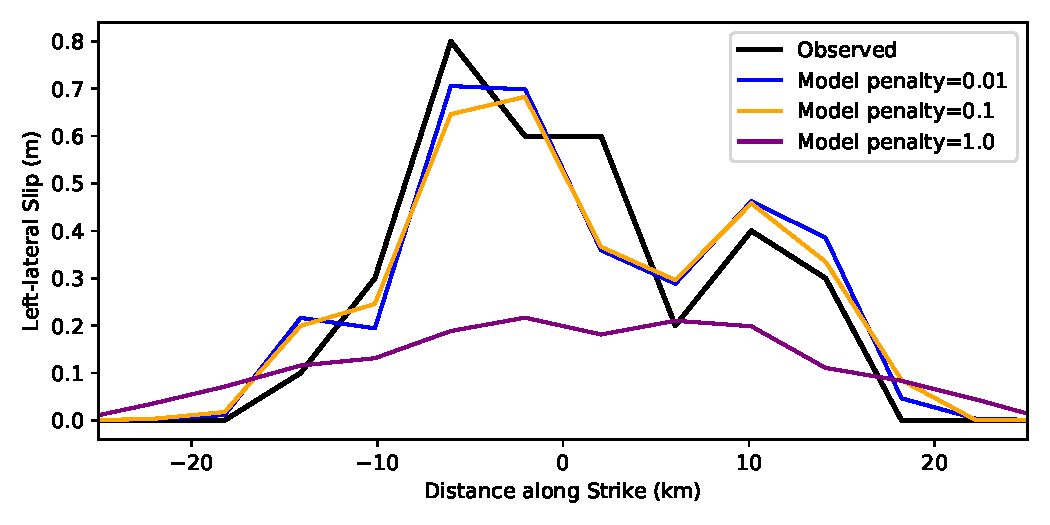
\includegraphics[height=6.1cm]{figs/step06-solution}
  \end{center}
  \vfill
  
\end{frame}

% ======================================================================
\end{document}


% End of file
